\doublespacing

\chapter{System Integration}
\label{ch3}

\begin{spacing}{1}
\minitoc
\end{spacing}
\thesisspacing

\section{Block Diagram explained}

\subsection{VDMA Block Diagram and System Integration}

This section explains the software reference renderer, camera-control path, stereoscopic output and integration of the hardware ray marcher into a complete HDMI pipeline. We first built the software renderer to give the group a working algorithmic reference. We then modified the initial BRAM framebuffer design into a double-buffered HDMI output path before implementing the full VDMA/DDR system: Vivado integration, a custom AXI DDR writer, Python control software, frame-swap handshaking and audio-reactive control registers.

The software reference renderer was built as a React application with CPU and GPU scaffold renderers, a shaded sphere renderer, a free-flight camera and a live performance HUD. The CPU renderer generates a camera ray for each pixel, evaluates the scaffold signed-distance field and writes the colour into a canvas \texttt{ImageData} buffer. It runs at the same $512 \times 300$ internal resolution as the FPGA, making the comparison meaningful. The GPU version evaluates the same scaffold shader in parallel using WebGL 2, confirming that the algorithm maps well to per-pixel parallelism. The shaded sphere scene, with normal estimation, lighting, soft shadows, ambient occlusion and fog, was used to validate the camera maths before reducing the hardware target to the simpler iteration-coloured scaffold.

We represented the camera using a 3D origin and a $3 \times 3$ orientation matrix rather than sending yaw and pitch directly into the FPGA. Yaw and pitch are convenient for user input, but converting them into rays requires trigonometric functions and vector normalisation, which are cheaper in Python than in RTL. The host therefore computes the camera basis, while the FPGA receives ready-to-use vectors for per-pixel ray generation.

The Pygame controller maintains yaw, pitch, position and movement speed. Yaw rotates the view around the vertical axis, while pitch controls the vertical component. The forward vector is:
\begin{equation}
\mathbf{f} =
\begin{bmatrix}
\sin(\text{yaw})\cos(\text{pitch}) \
\sin(\text{pitch}) \
-\cos(\text{yaw})\cos(\text{pitch})
\end{bmatrix}.
\end{equation}

Here, $\sin(\text{pitch})$ gives the vertical component and $\cos(\text{pitch})$ gives the remaining horizontal length. Yaw splits this horizontal component between $x$ and $z$ using $\sin(\text{yaw})$ and $-\cos(\text{yaw})$, giving a unit-length forward vector without an extra host-side normalisation step.

The right vector is:
\begin{equation}
\mathbf{r} =
\begin{bmatrix}
\cos(\text{yaw}) \
0 \
\sin(\text{yaw})
\end{bmatrix}.
\end{equation}

This is perpendicular to the horizontal projection of the forward vector and has no $y$ component, so strafing stays level even when the user looks up or down. The up vector is calculated from the cross product of the right and forward vectors, completing an orthogonal camera frame.

These three vectors form the camera matrix:
\begin{equation}
M =
\begin{bmatrix}
r_x & u_x & f_x \\
r_y & u_y & f_y \\
r_z & u_z & f_z
\end{bmatrix}.
\end{equation}

A camera-space ray is rotated into world space by:
\begin{equation}
\mathbf{d}_{world}=d_x\mathbf{r}+d_y\mathbf{u}+d_z\mathbf{f}.
\end{equation}

A centre pixel has almost no right or up offset, so its ray points mainly along the forward vector. A top-right pixel has positive right and up offsets, so its ray becomes a weighted mixture of the right, up and forward vectors. This keeps the FPGA calculation simple while still allowing arbitrary camera orientation.

In hardware, the Pygame controller sends twelve 32-bit floating-point values over TCP: nine camera-matrix entries and three origin coordinates. On the PYNQ, the Python service converts each IEEE-754 value into the RTL's 27-bit floating-point format and writes it into the AXI-Lite camera register file. The conversion keeps the sign bit and 8-bit exponent, but rounds the mantissa to 18 bits. This preserves useful dynamic range while reducing FPGA arithmetic width. The same AXI-Lite interface also carries DDR framebuffer addresses and scene-control parameters.

The ray-generation module converts each incoming pixel coordinate into a camera-space ray. The $x$ and $y$ coordinates give horizontal and vertical offsets from the centre of the eye image, while a fixed forward-depth constant controls the field of view. These offsets are converted to 27-bit floating point, squared, summed and passed through the inverse-square-root block to normalise the ray. The design then applies the camera matrix using nine floating-point multiplications and six additions, with pipeline delays keeping camera data, pixel ID and ray components aligned.

The same camera system was extended for stereoscopic output. The rendered $512 \times 300$ internal frame is split into two 256-pixel-wide eye images. For the right eye, the ray generator subtracts 256 from the $x$ coordinate so each half has its own local screen coordinate system. The march core forms the eye origins by offsetting the camera origin along the right vector:
\begin{equation}
\mathbf{origin}_{left} = \mathbf{origin} - \mathbf{r}\cdot\text{half\_IPD}
\end{equation}
and the right-eye origin is:
\begin{equation}
\mathbf{origin}_{right} = \mathbf{origin} + \mathbf{r}\cdot\text{half\_IPD}.
\end{equation}

Both eyes use the same orientation matrix, but their origins are laterally separated. This produces the horizontal parallax needed for stereoscopic 3D while reusing the same ray-marching pipeline for both halves of the image.

The first FPGA display path used BRAM as the framebuffer. We modified it into a double-buffered design because a single framebuffer was unsafe when the renderer and HDMI scan-out operated concurrently. One BRAM bank was written by the render pipeline while the other was read by scan-out. The two buffers were stored back-to-back, with the write address offset by 153,600 when the render bank was high. The displayed bank changed only on vertical sync, preventing mid-frame buffer switches.

The BRAM scan-out path mapped the $512 \times 300$ internal render to $1024 \times 600$ HDMI output by duplicating each pixel horizontally and vertically. This kept the workload at 153,600 rays per frame while filling the headset display. The BRAM version was useful for debugging, but it used 120 out of 140 Block RAM tiles, or 85.71%, making the framebuffer the dominant resource constraint.

\begin{figure}[htbp]
\centering
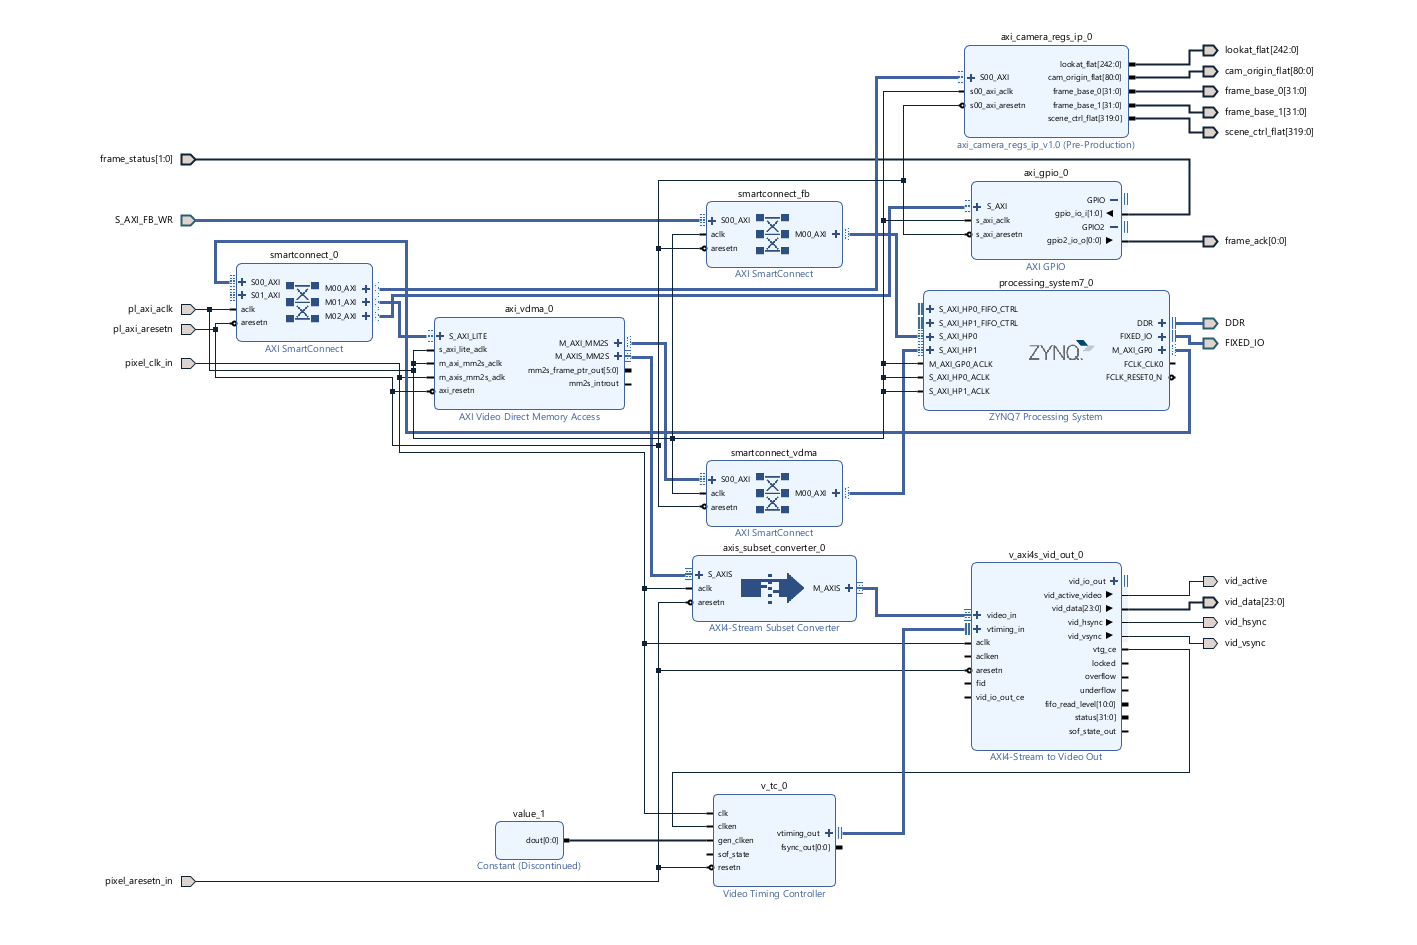
\includegraphics[width=0.95\linewidth]{imgs/vdma_block_diagram.png}
\caption{Vivado block diagram for the VDMA-based HDMI output architecture. The design separates low-bandwidth AXI-Lite control traffic from high-bandwidth frame-buffer traffic through DDR.}
\label{fig:vdma-block-diagram}
\end{figure}

The VDMA version replaced the BRAM framebuffer with two frame buffers in external DDR. Figure~\ref{fig:vdma-block-diagram} shows the final Vivado block design, built around the Zynq processing system, custom accelerator IP, AXI VDMA, AXI GPIO, video timing controller, AXI4-Stream-to-video-out, AXI-stream subset conversion, RGB-to-DVI and SmartConnect blocks. GP0 handles low-bandwidth AXI-Lite control, including the camera/scene registers at \texttt{0x43C00000}, VDMA control at \texttt{0x43000000} and GPIO at \texttt{0x41200000}. The high-bandwidth frame paths are separate: the custom writer reaches DDR through HP0, while the VDMA reads display frames through HP1. The CPU configures the system and swaps buffers, but never transfers pixels itself.

The VDMA is configured only in memory-to-stream mode because the FPGA writes rendered frames using its own AXI master. The PYNQ software allocates two non-cacheable $1024 \times 600$ \texttt{uint32} buffers in DDR and writes their physical addresses into both the VDMA start-address registers and accelerator framebuffer-base registers. The VDMA uses a 4096-byte horizontal size, 4096-byte stride and 600 lines, matching a $1024 \times 600$ frame with 32 bits per pixel. It runs in park mode so software can choose which buffer is displayed. The VDMA stream then passes through the video output path, where the 24 RGB bits are extracted before HDMI output.

The custom DDR writer receives completed ray results as a pixel ID and 8-bit iteration count. The palette converts this to 24-bit RGB, then the render bank, pixel ID and colour are packed into a 45-bit FIFO entry. The 4096-entry FIFO isolates the ray-marching pipeline from the AXI write interface: if DDR writes stall, completed pixels accumulate; if the FIFO approaches full, the top-level controller stalls new dispatch before data is lost.

The DDR writer also performs the $2 \times 2$ scaling from $512 \times 300$ render resolution to $1024 \times 600$ display resolution. Each internal result at $(x,y)$ becomes four output pixels. Rather than issuing four separate 32-bit writes, each horizontal pair is packed into one 64-bit AXI beat:
\begin{equation}
{\texttt{8'h00},\ \texttt{rgb},\ \texttt{8'h00},\ \texttt{rgb}}.
\end{equation}
Repeating this write one display row lower reduces each internal pixel to two 64-bit writes and uses the full HP0 data width.

The DDR frame is linear, with 1024 pixels per row and 4 bytes per pixel, so each output row occupies 4096 bytes. Each internal row expands into two output rows and each internal column into two 32-bit output pixels, so the top-row address is:
\begin{equation}
\mathrm{addr}_{top}=\mathrm{base}+(y \times 8192)+(x \times 8).
\end{equation}

This maps naturally to hardware shifts because $y \times 8192$ is a left shift by 13 and $x \times 8$ is a left shift by 3. The second row of the $2 \times 2$ block is written by adding 4096 bytes. The resulting layout is exactly what the VDMA expects: a normal $1024 \times 600$, 32-bit-per-pixel linear frame.

The writer uses AXI single-beat incrementing writes. \texttt{AWLEN} is zero, \texttt{AWSIZE} selects an 8-byte beat, \texttt{AWBURST} is incrementing and all byte strobes are enabled. Address and data channels are independent, so the writer keeps separate \texttt{w\_sent} and \texttt{w\_sent} flags, treats a beat as issued only once both handshakes complete and tracks B-channel responses with an outstanding-response counter. Up to eight outstanding writes are allowed, so the design does not assume a write has reached DDR simply because address and data were accepted by the interconnect.

Frame completion is controlled carefully. Dispatch stops after 153,600 internal rays have been issued, and completion is detected when 153,600 results return. However, the frame is not handed to the VDMA until the DDR writer is drained. This signal is asserted only when the result FIFO is empty, no active or prefetched entry remains, no beat is in progress, no delayed pixel is entering the writer and all outstanding write responses have returned. This ensures all pixels are safely visible in DDR before display.

Frame ownership is handled using AXI GPIO. Channel 1 carries frame-ready and completed-bank status bits from FPGA to Python, while Channel 2 carries the acknowledgement bit back. When a frame is drained, Python parks the VDMA on the completed bank and pulses acknowledgement for 1 ms. The FPGA then clears ready, toggles the render bank and starts the next frame. This prevents displaying an incomplete buffer or overwriting one still being displayed.

The Python control flow maps the camera register IP, VDMA and GPIO through MMIO, allocates two DDR frame buffers, writes default camera and scene values, writes framebuffer addresses to the accelerator and configures the VDMA. It also services the frame-ready handshake during camera socket timeouts, so display updates continue even when camera input is idle. Audio-reactive scene parameters are written through the same control path and latched at frame boundaries so each frame uses a consistent scene state.

The measured performance and resource results show the architectural trade-off. The CPU scaffold renderer averages approximately 1.2 FPS at $512 \times 300$, while the FPGA scaffold scene averages approximately 18.46 FPS after the VDMA/frame-ready handshake, corresponding to 54.22 ms per frame and a $15.4\times$ improvement by FPS. Moving from BRAM to DDR reduced framebuffer BRAM usage from 120 tiles to 3 tiles, at the cost of extra LUT, register and DSP usage from the AXI writer, DDR interconnect, VDMA path and control structure.

\subsection{Implementation utilisation and timing}

Table~\ref{tab:impl-utilisation} summarises post-implementation resource utilisation for the final VDMA design. The key result is low BRAM usage: only 3 out of 140 BRAM tiles, or 2.14%.

\begin{table}[htbp]
\centering
\caption{Post-implementation resource utilisation for the final VDMA design.}
\label{tab:impl_utilisation}
\begin{tabular}{|l|r|r|r|}
\hline
Resource & Used & Available & Utilisation \\
\hline
Slice LUTs & 22,366 & 53,200 & 42.04\% \\
Slice registers & 13,499 & 106,400 & 12.69\% \\
Slices & 6,844 & 13,300 & 51.46\% \\
BRAM tiles & 3 & 140 & 2.14\% \\
DSP48E1 & 62 & 220 & 28.18\% \\
Bonded IOB & 10 & 125 & 8.00\% \\
BUFGCTRL & 4 & 32 & 12.50\% \\
MMCM & 1 & 4 & 25.00\% \\
\hline
\end{tabular}
\end{table}

The post-route timing report showed that all specified constraints were met. The worst setup slack was 0.123 ns and the worst hold slack was 0.016 ns, with no failing setup or hold endpoints. The design was valid after implementation, although the small margins show that the final VDMA build was close to the timing limit.

\begin{table}[htbp]
\centering
\caption{Post-route timing summary for the final VDMA design.}
\label{tab:timing_summary}
\begin{tabular}{|l|r|}
\hline
Timing metric & Value \\
\hline
Setup WNS & 0.123 ns \\
Setup TNS & 0.000 ns \\
Setup failing endpoints & 0 \\
Hold WHS & 0.016 ns \\
Hold THS & 0.000 ns \\
Hold failing endpoints & 0 \\
Pulse-width worst slack & 1.740 ns \\
Routed nets with errors & 0 \\
\hline
\end{tabular}
\end{table}

The main implementation clock was \verb|clk_out1_clk_wiz_0| at 140.016 MHz. The design also used \verb|clk_out2_clk_wiz_0| at 51.339 MHz for the video path and \verb|clk_out3_clk_wiz_0| at 256.696 MHz with few loads. Four global clock buffers and one MMCM were used. The routed design contained 30,837 routable nets, all fully routed with no errors.

\section{UI and Bitstream Switching}

Crucial to our design, we wanted to be able to switch scenes through a UI. Given the high LUT usage, and that each signed distance function counts for at minimum 3,000 LUTs, it was unfeasible to have all SDFs on one bitstream. Bitstream switching had to be developped.

\subsection{Scene Selector}

The graphical scene selector is rendered directly into a VDMA-backed DDR3
framebuffer and displayed over the same HDMI output as the ray marcher,
eliminating the need for a separate display or serial terminal. The UI is
implemented in Python on the PYNQ Linux stack (\texttt{selector.py}) and
runs on a dedicated \texttt{ui.bit} bitstream whose sole purpose is to drive
the VDMA and accept button input; no ray marching hardware is loaded
during menu navigation.

A pre-rendered PNG (\texttt{base\_ui.png}) is loaded once at startup,
converted to a $1024\times600$ NumPy array, and packed into the 32-bit-per-pixel
format expected by the VDMA (\texttt{0x00RRGGBB}). On each frame, Pillow
draws a highlight rectangle over the currently selected scene entry and
redraws the music-enable indicator, then writes the result directly into the
physically-addressed DDR3 framebuffer via NumPy array assignment --- no
intermediate copy, no DMA transaction from the PS side.

\begin{lstlisting}[language=Python]
def _to_uint32(img_array):
    arr = img_array.astype(np.uint32)
    return (arr[:,:,0] << 16) | (arr[:,:,1] << 8) | arr[:,:,2]

def render_frame(base, selected, music_on, framebuf):
    img  = Image.fromarray(base.copy())
    draw = ImageDraw.Draw(img)
    y    = OPTION_Y[selected]
    draw.rectangle([HIGHLIGHT_X[0], y - HIGHLIGHT_H,
                    HIGHLIGHT_X[1], y + HIGHLIGHT_H],
                   outline=(255, 50, 200), width=3)
    framebuf[:] = _to_uint32(np.array(img))
\end{lstlisting}

Three on-board push-buttons are read by polling an AXI GPIO IP at
\texttt{0x41210000}: BTN1 scrolls down, BTN2 scrolls up, BTN3 confirms
(short press) or toggles music reactivity (long press, $>$0.5\,s). A
software debouncer spins until the button is released then waits 50\,ms
before re-enabling input, preventing repeated triggering from contact bounce.

\subsection{Runtime Bitstream Switching}

Selecting a scene triggers a runtime bitstream swap via PYNQ's
\texttt{Overlay} API, which reconfigures the entire PL fabric without
rebooting the PS or interrupting the Linux stack. This took days to integrate and relies on a neat trick of dropping pixel HDMI frequency to cause a VDMA reset. The system initially worked fine but the screen would shift right by random amounts, due to improper resets of VDMA buffer. The out of sync frequency solved that issue. The swap sequence is:

\begin{enumerate}
\item Write \texttt{DMACR\,=\,0x00} to the VDMA to stop pixel output
      immediately, preventing the HDMI serialiser from receiving partial
      or garbage pixel data during reconfiguration.
\item Lower \texttt{FCLK0} to 15\,MHz via \texttt{pynq.Clocks}. The
      clock wizard downstream of FCLK0 loses lock and the HDMI pixel clock
      drops, causing the monitor to report \textit{no signal} cleanly rather
      than displaying noise.
\item Call \texttt{Overlay(bitfile)}, which takes 3--5\,s to write the new
      bitstream to the FPGA configuration port. The Overlay parser reads the
      hardware handoff file (\texttt{.hwh}) to restore FCLK0 for UI
      bitstreams automatically.
\item For SDF bitstreams, restore \texttt{FCLK0\,=\,50\,MHz} manually so
      the clock wizard generates 125\,MHz from this reference. The 50\,ms
      sleep that follows allows the MMCM to re-lock before AXI traffic
      begins.
\item Re-initialise VDMA, allocate two DDR3 framebuffers, write frame base
      addresses to the AXI camera register file, and start the ray marcher
      loop.
\end{enumerate}

\begin{lstlisting}[language=Python]
def pl_hdmi_load(bitfile, min_dark_sec=0):
    MMIO(0x43000000, 0x10000).write(0x00, 0x00)  # stop VDMA
    time.sleep(0.01)
    Clocks.fclk0_mhz = 15.0          # HDMI pixel clock drops -> no signal
    t0  = time.monotonic()
    ol  = Overlay(bitfile)            # ~3-5s reconfiguration
    remaining = min_dark_sec - (time.monotonic() - t0)
    if remaining > 0:
        time.sleep(remaining)
    return ol
\end{lstlisting}

The total dark interval on the monitor is \texttt{max(min\_dark\_sec,
Overlay\_time)} rather than their sum. The FCLK0 drop and
\texttt{Overlay()} call overlap, so no additional sleep is added unless the
bitstream loads faster than the minimum dark window.

After the ray marcher finishes (user presses BTN1 to return to menu), the
same sequence runs in reverse: VDMA stopped, FCLK0 lowered,
\texttt{ui.bit} loaded, VDMA reinitialised on the UI framebuffer, and the
selector loop resumes with the highlight on the previously selected scene.
The full round-trip, scene exit to menu reappearing, takes
approximately 6--8\,s, dominated by the two \texttt{Overlay()} calls.

\begin{figure}[htbp]
    \centering
    % Top Image (Rotated 90 degrees anticlockwise)
    \begin{minipage}[b]{\textwidth}
        \centering
        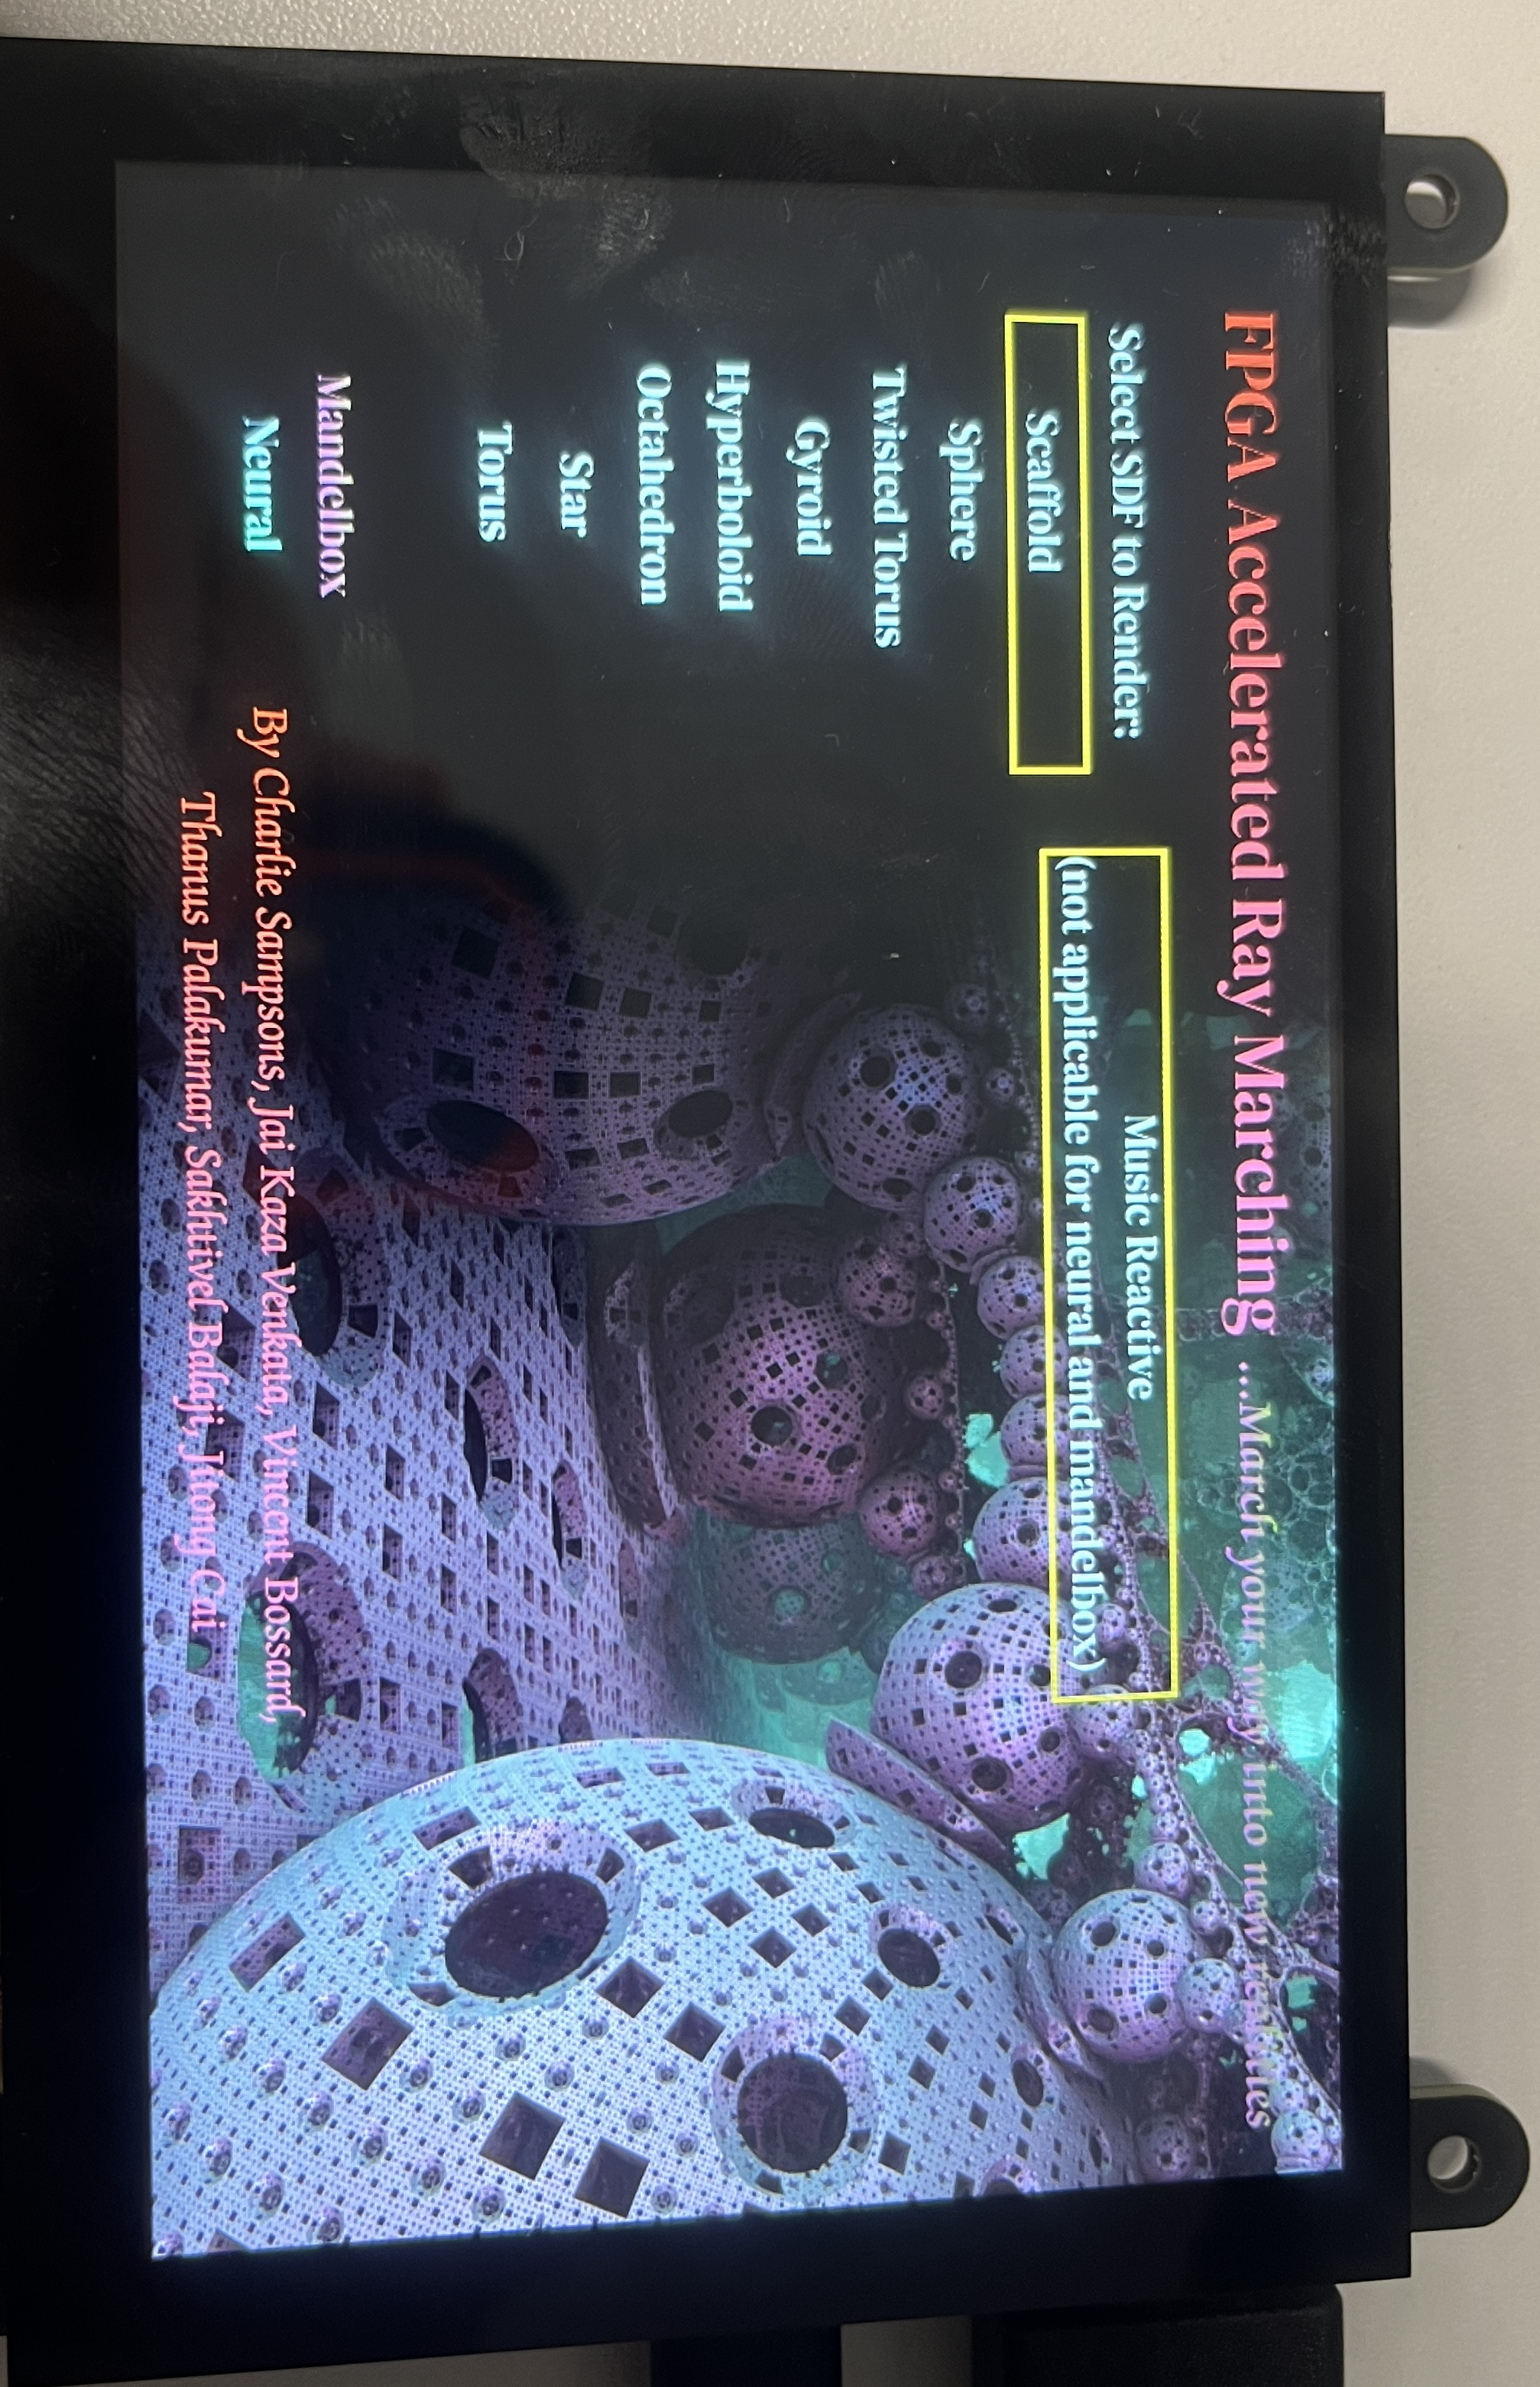
\includegraphics[width=0.3\textwidth,angle=90]{imgs/ui_no_shift.jpg}
        \label{fig:image1}
    \end{minipage}
    
    \vspace{15pt} % Adds clean breathing room between the two vertical images
    
    % Bottom Image (Rotated 90 degrees anticlockwise)
    \begin{minipage}[b]{\textwidth}
        \centering
        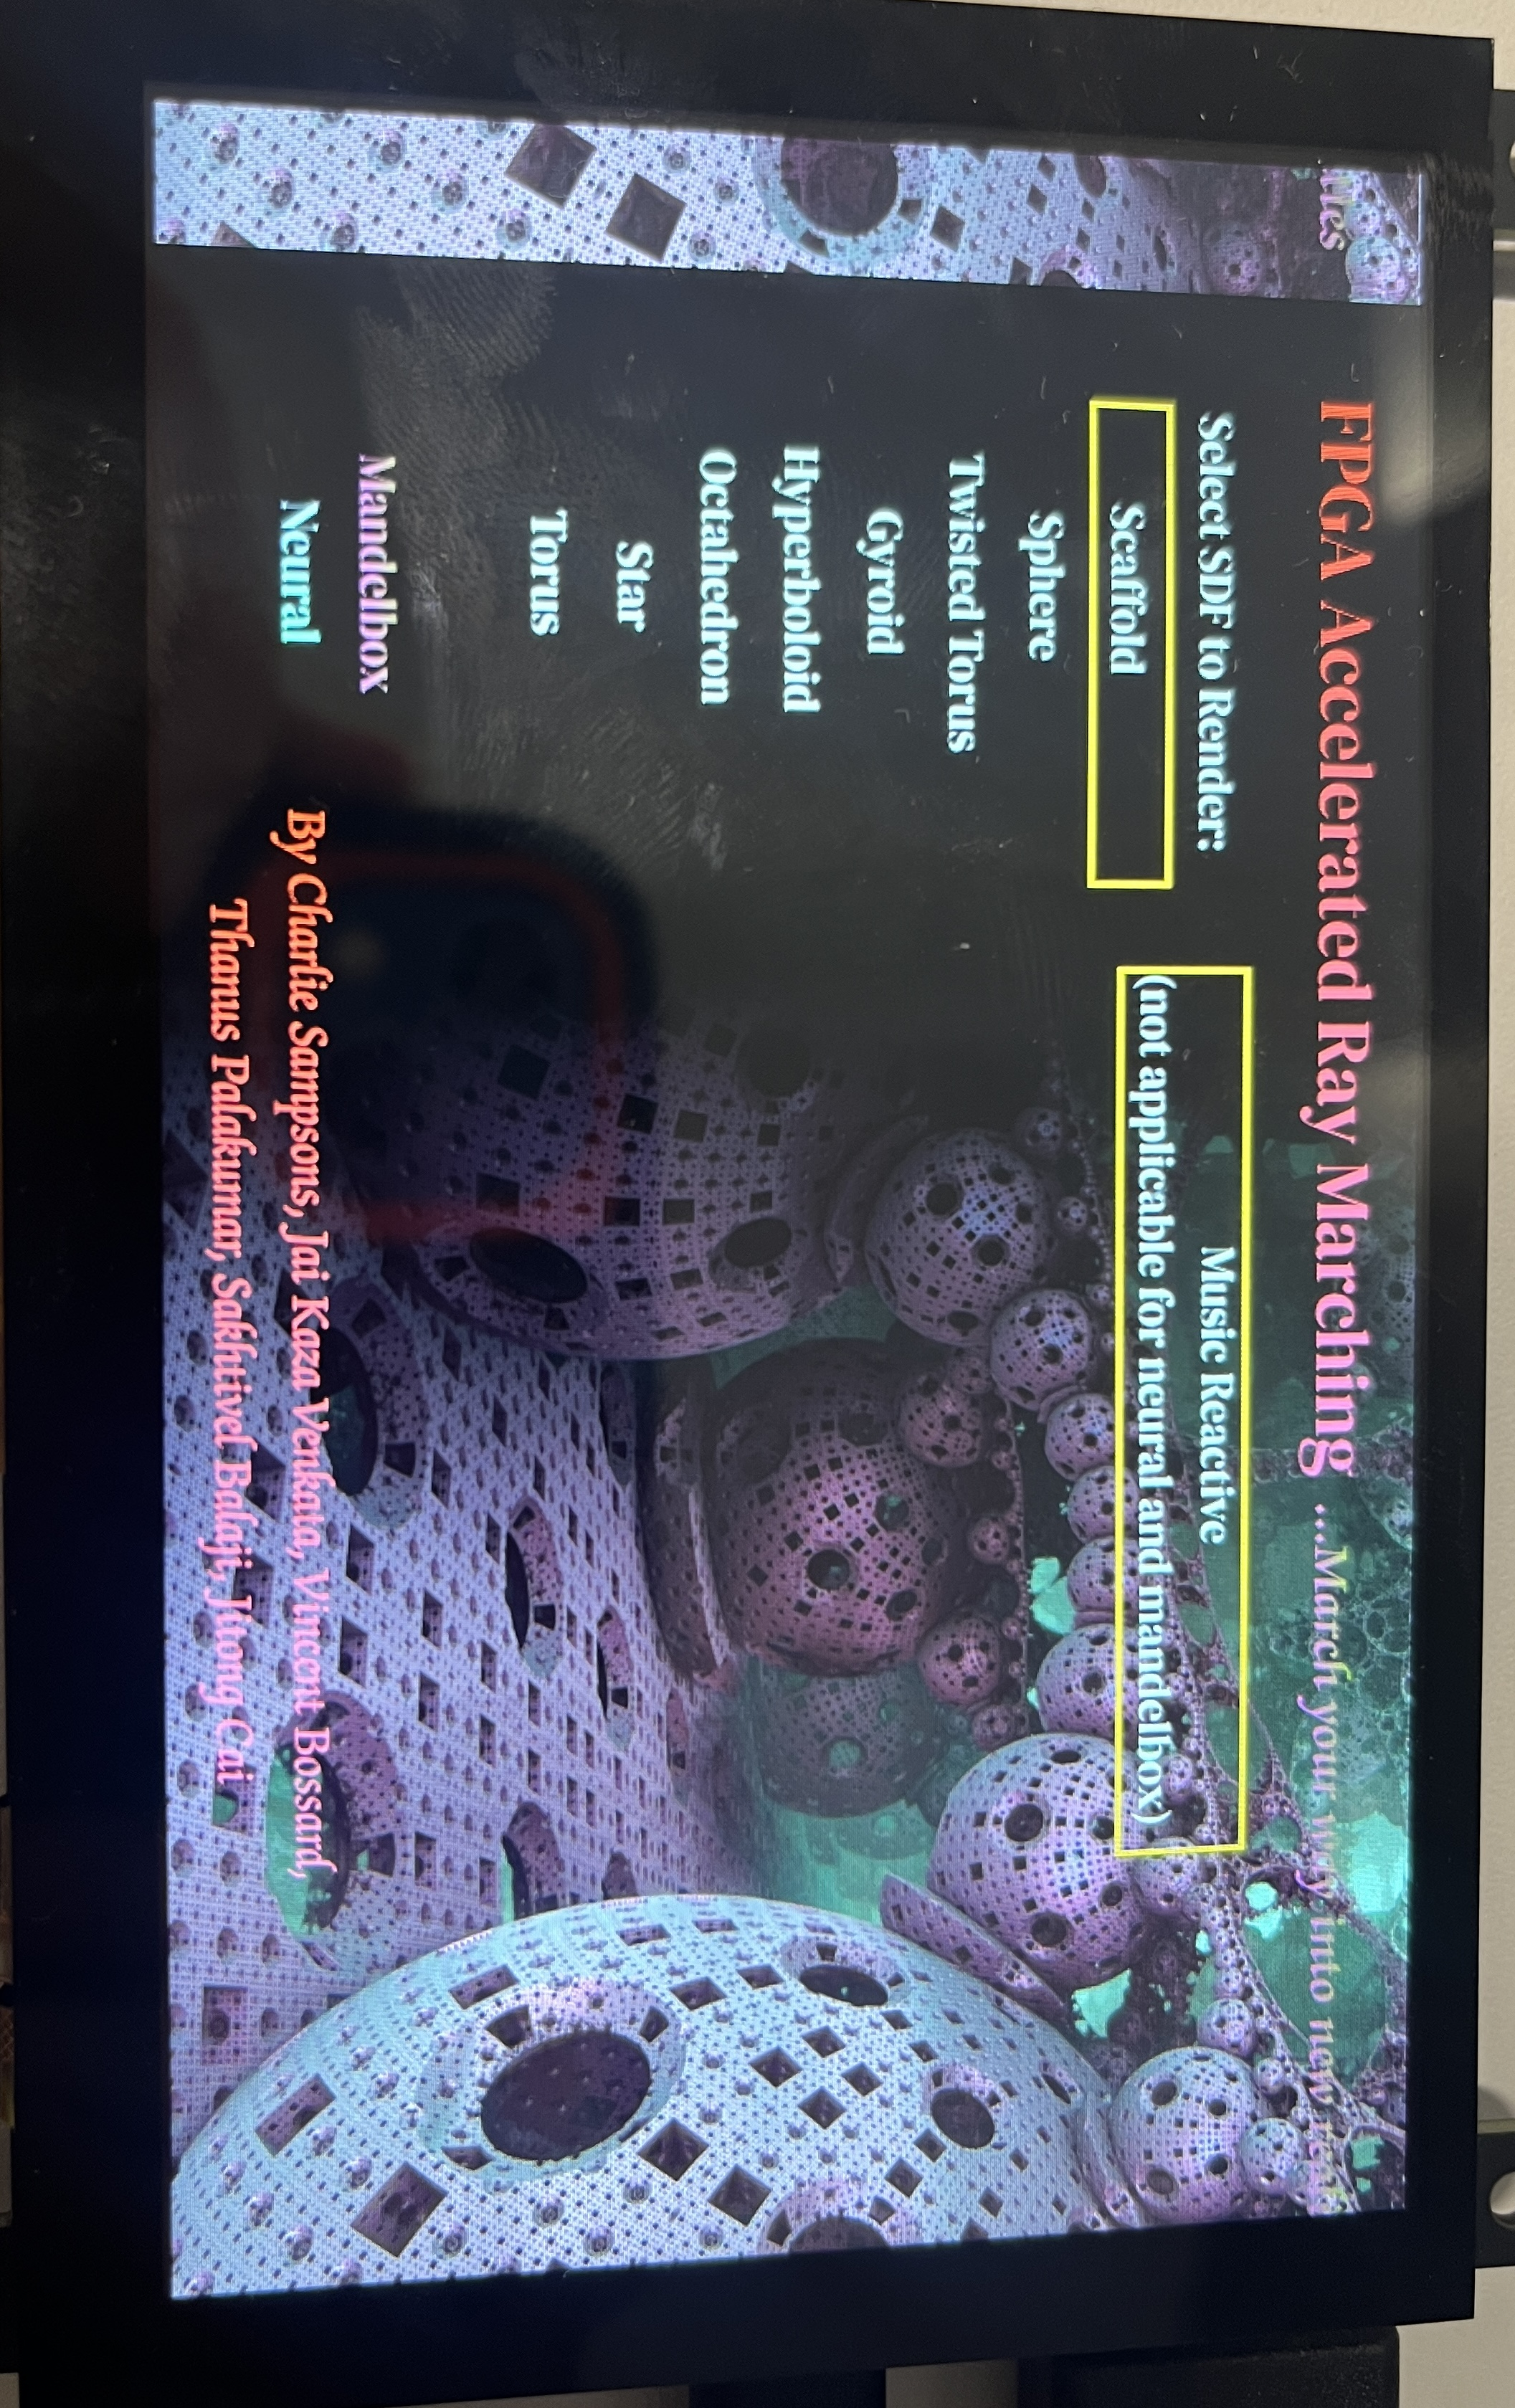
\includegraphics[width=0.3\textwidth,angle=90]{imgs/ui_shifted.jpg}
        \label{fig:image1000}
    \end{minipage}
    
    \caption{Base UI. Rectangles are drawn by PIL / Pillow library on top of the base UI screen. The right image shows the random shift that contaminated UI and scenes, due to incomplete reset of VDMA buffer.}
\end{figure}

\section{3D printed VR headset}
% ==============================================================================
% 1. VR HEADSET % ==============================================================================

As a group, we wanted to improve the interactivity of our design, so we decided on building a VR headset so the user can really interact with our outputs, and because of my experience in CAD, a lot of time was spent designing our headset and 3D printing it.

Instead of designing one completely from scratch, we made use of an open source DIY design called \textit{Relativity} (\url{https://github.com/relativty/Relativty/tree/master}) as a base. However, this was obviously not designed for an FPGA or the screen we had to order due to time and budget constraints, which led us to construct a major redesign of this base. We had to consider our requirements, which was that the headset had to be able to securely hold a Pynq FPGA, mount the screen and maintain a 45mm focal length of our lenses.

\subsection{Lens Mount Modifications}
Our project used custom 37mm diameter biconvex lenses. The original Relativity eye holes were the wrong size for these so we remodelled the inner lens cups, making sure the diameter was toleranced correctly so the 37mm lenses could be friction-fitted securely into the plastic. This meant we didn't have to use glue, which was important since that could easily ruin the lenses. The original design made use of smaller lenses, while the larger lenses we purchased were because we expected them to give a slightly better FOV. 

\begin{figure}[htbp]
    \centering
    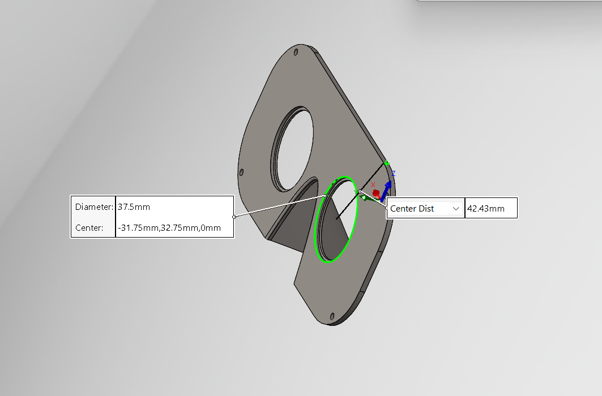
\includegraphics[width=0.8\textwidth]{imgs/Headset_Images/lens_mount.png} 
    \caption{Modifications made to the lens mount to accommodate the custom 37mm biconvex lenses.}
    \label{fig:lens_mount}
\end{figure}

\subsection{Screen Panel Overhaul and Focal Length Geometry}
This was one of the more difficult mechanical challenges. The lenses we bought had a strict 45mm focal length but the original Relativity CAD was designed for a dual-screen setup mounted directly in front of the middle panel. However, we were using a single, larger 5-inch screen.

Because of the physical size of our screen, we had to create entirely new geometry. We removed the dual-screen mount and redid almost the entire screen panel. To make the 5-inch screen fit properly, it had to be mounted behind the panel rather than in front of it which changed the focal length, so we had to iteratively redesign the depth of the entire headset body. We calculated the exact distance to the LCD panel and adjusted the extrusions until the screen sat exactly at the 45mm focal point. Also because the screen fit so tightly, we had to account for cabling in advance by creating space for a 90-degree HDMI cable so the wiring wouldn't hit the side walls of the headset.

\begin{figure}[htbp]
    \centering
    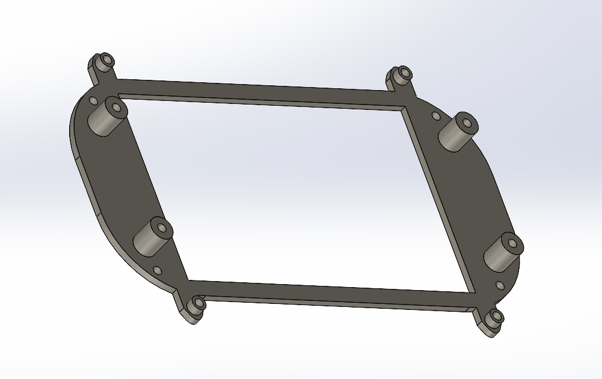
\includegraphics[width=0.8\textwidth]{imgs/Headset_Images/screen_panel.png}
    \caption{Redesign of the screen panel geometry to achieve the exact 45mm focal length for a single 5-inch screen.}
    \label{fig:screen_panel}
\end{figure}

\begin{figure}[htbp]
    \centering
    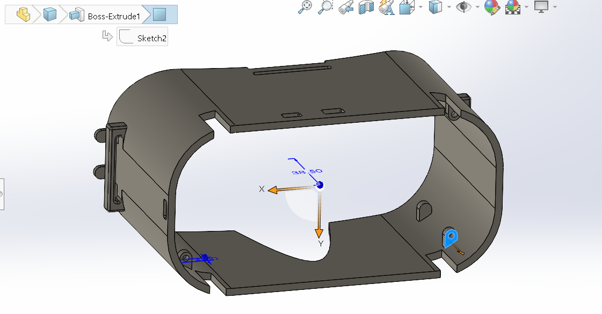
\includegraphics[width=0.8\textwidth]{imgs/Headset_Images/body.png}
    \caption{Final modified body geometry after screen panel and focal length adjustments.}
    \label{fig:body}
\end{figure}

\subsection{Quest 2 Headstrap Integration}
Another physical constraint of our project was weight. Strapping a PCB, an FPGA, and an LCD screen to someone's face makes the headset quite front-heavy and the original Relativity model only had thin slots for generic velcro straps, which would have been uncomfortable. We bought a generic Meta Quest 2 headstrap which our model didn't have the option for, but the Quest 2 straps would give better security for our headset which will be quite heavy due to the FPGA as well. 

Because our CAD obviously didn't have the specific snapping geometry needed for a Quest 2 strap, we modified and made use of an existing adapter model online for a Quest 3 to Quest 2. Firstly, we deleted the original vertical velcro loop and mated the adapter arm further forward toward the screen to clear the screw holes for the foam support panel. We then modified the geometry of the adapter arms by getting rid of the Quest 3 section and mating just the Quest 2 part to the main body.

\begin{figure}[htbp]
    \centering
    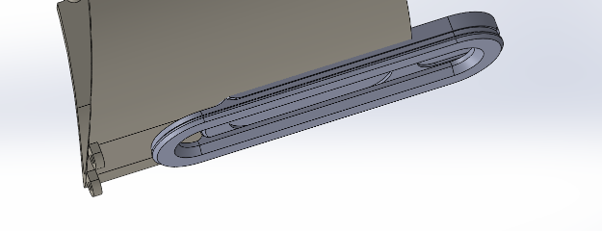
\includegraphics[width=0.8\textwidth]{imgs/Headset_Images/quest2_strap_1.png}
    \caption{Modified adapter arms integrated into the main body (Image 1).}
    \label{fig:quest2_strap_1}
\end{figure}

\begin{figure}[htbp]
    \centering
    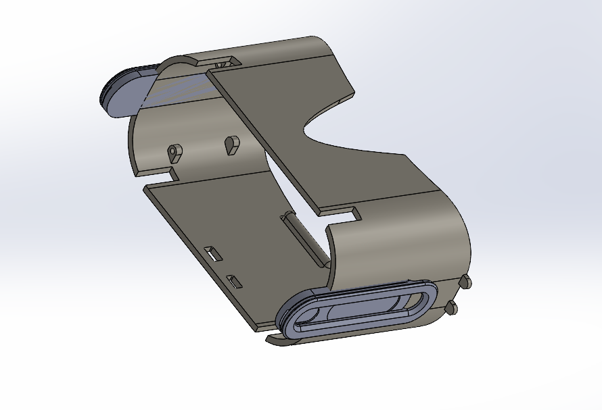
\includegraphics[width=0.8\textwidth]{imgs/Headset_Images/quest2_strap_2.png}
    \caption{Modified adapter arms integrated into the main body (Image 2).}
    \label{fig:quest2_strap_2}
\end{figure}

\subsection{FPGA Housing, IMU Bracket, and Friction Fit}
To accommodate for the FPGA we had to increase the length of the main body so we could fit another panel in front of it which will help block out light. The FPGA comes in an unremovable 3D printed case, and the dimensions of it are 126 by 91mm.

Rather than using screws, we designed the cavity's internal dimensions with an extra 0.5mm to 1mm tolerance to implement a friction fit for the entire 126x91mm case. The FPGA case snaps securely into the front of the headset. 

\begin{figure}[htbp]
    \centering
    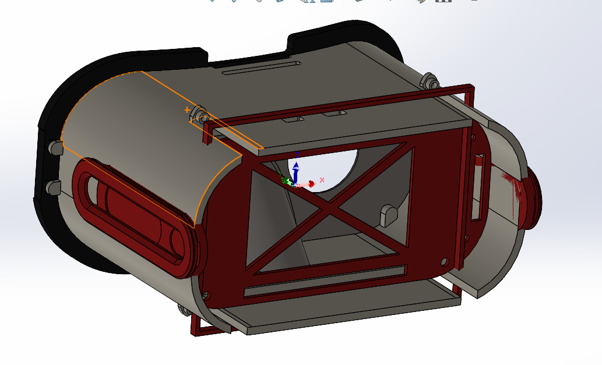
\includegraphics[width=0.8\textwidth]{imgs/Headset_Images/fpga_housing_1.png}
    \caption{CAD model demonstrating the friction fit dimensions for the FPGA housing.}
    \label{fig:fpga_housing_1}
\end{figure}

Finally, on this front plate, we also added a custom mounting bracket for our MPU-9250 IMU sensor, and 3D printed some 4mm standoffs to make sure the sensor sat perfectly level to get accurate head-tracking data.

\begin{figure}[htbp]
    \centering
    
\includegraphics[width=0.8\textwidth]{imgs/Headset_Images/most_front_panel.png}
    \caption{Front panel showcasing the custom mounting bracket and standoffs for the IMU sensor.}
    \label{fig:most_front_panel}
\end{figure}

The above image was obviously modified in order to provide space for the FPGA as you can see there is an overlap right now. We then generated a nice final rendered image so we can see exactly what we will be building, which was made using SOLIDWORKS Visualize.

\begin{figure}[htbp]
    \centering
    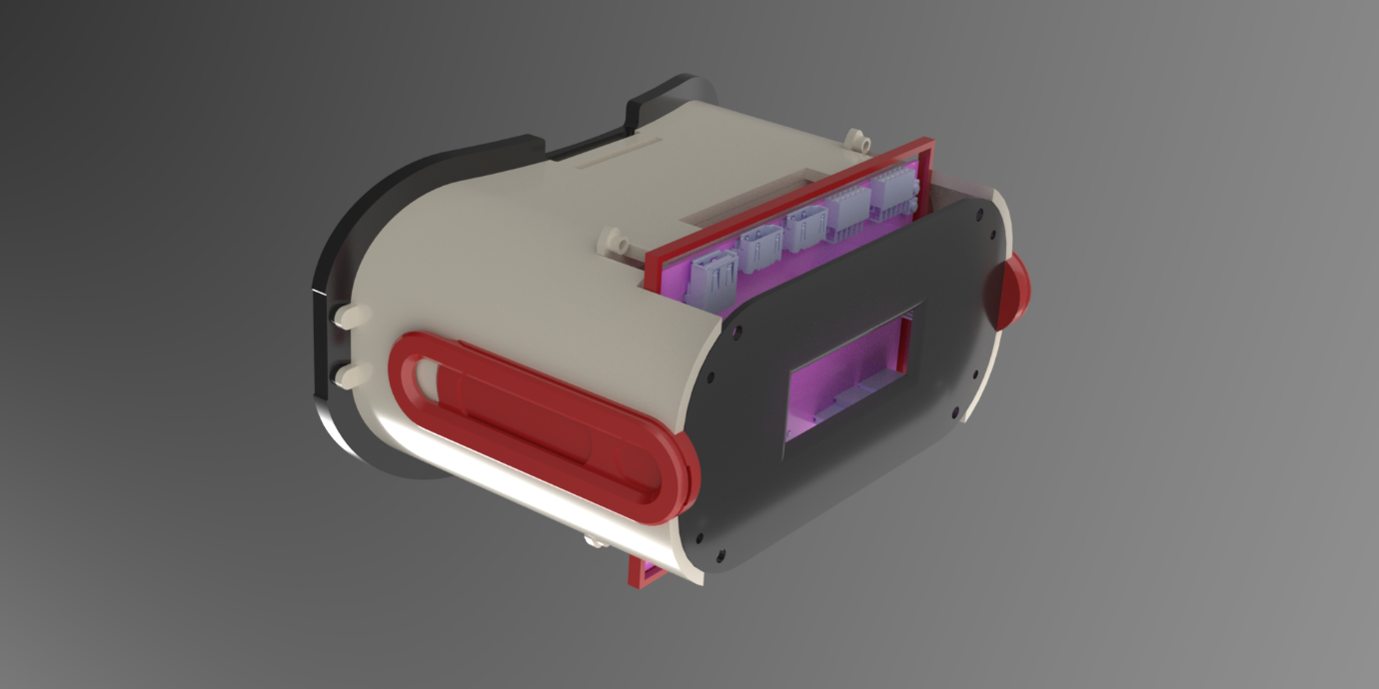
\includegraphics[width=0.8\textwidth]{imgs/Headset_Images/final_rendered.png}
    \caption{Final rendered image of the VR headset design generated in SOLIDWORKS Visualize.}
    \label{fig:final_rendered}
\end{figure}

After designing, we 3D printed all of our parts, and began construction. This phase, included testing and also due IO placement on the screen and FPGA, some minor re-designs that led to re-printing, such as extra space for the HDMI cable.

\begin{figure}[htbp]
    \centering
    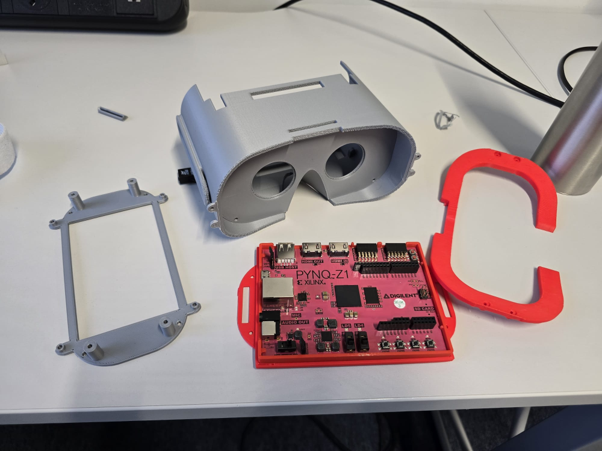
\includegraphics[width=0.8\textwidth]{imgs/Headset_Images/physical_construction.png}
    \caption{Starting the physical construction of the 3D-printed VR headset.}
    \label{fig:physical_construction}
\end{figure}
